
\section{Introduction}

Alongside genomic analysis, we developed and employed other "omics" techniques to enhance our understanding of key biological aspects of \ac{Focub} infection and to support the diagnosis of \ac{fwb}. Omics, is defined by \textcite{Dai2022}, as "probing and analysing large datasets representing the structure and function of an entire biological system at a specific level". Numerous omics approaches, including genomics, transcriptomics, proteomics, metabolomics, and phenomics, have emerged in recent decades and have been instrumental in studying plants and their associated biotic and abiotic stresses. Indeed, \textcite{Backiyarani2022} provide a comprehensive review of omics techniques applied in banana research and their contributions to banana improvement. We are witnessing a transition into the era of "multi-omics", where these techniques and datasets are integrated to uncover novel associations between biological systems at various levels \parencite{Hasin2017}.

The adoption of multi-omics approaches for investigating plant diseases has become increasingly prevalent. For example, \textcite{Crandall2020} illustrate how both metabolomics and genomics have deepened our understanding of the salicylic acid pathway's role in plant defence. \textcite{Zhu2021} employed transcriptomics and metabolomics to explore the effects of different soil treatments on \ac{Fo} \ac{fsp} \textit{capsici} infestation in pepper (\textit{Capsicum annuum}). In our study, we employed phenomic analyses, including multispectral and RGB imaging, and \acf{um} analysis, to elucidate banana responses to various wilting stresses and help develop \ac{fwb} disease diagnostic methods.


Multispectral and RGB imaging studies in banana been established for disease detection and diagnosis. \textcite{Johansen2014} developed an automatic banana identification software to aid in Banana Bunch Top Virus inspection and \textcite{Liao2018} employed hyperspectral images and machine learning to diagnose Banana Streak Virus at earlier stages of infection. \textcite{Ochoa2016} designed a hyperspectral imaging system for disease scanning on banana plants focusing on Black Sigatoka. \acp{uav}, RGB imaging, and Artificial Neural Networks have also been employed in the monitoring of Yellow Sigatoka \parencite{Calou2020}.  

Recently, \acf{rs} disease diagnosis efforts in banana have focused on the identification of \ac{Focub} infection \parencite{Ye2020a, Ye2020b, Selvaraj2019}.  Ye et al (2020a,b) demonstrated that \ac{uav}-based multispectral imagery can be used to diagnose \ac{fwb}. The authors observed statistically significant differences (p > 0.05) between healthy and diseased plants using six different \acp{vi}. Using logistic regression models to describe the relationship between the \acp{vi} in healthy or diseased plants, the authors reported that the red-edge chlorophyll index had the best performance for identifying \ac{fwb}.  

It is clear that spectral reflectance can be used to diagnose \ac{fwb} in banana. What is not clear, however, is what is happening from a biological perspective to cause the differences in spectra observed, and whether the changes in spectra can be distinguished from other biotic and abiotic stresses. For instance, as \ac{Focub} is a vascular pathogen, it is important to ensure that \ac{Focub} infection can be differentiated from drought stress and other vasucular wilt pathogens like \acf{xvm}. 

Metabolomics, another vital "omics" field used in biological sciences, is the comprehensive analysis of the spectrum of metabolites within a biological system \parencite{Klassen2017}. Frequently used to track disease progression and pinpoint potential novel metabolites associated with disease and disease susceptibility; metabolomics has become a useful tool in disease diagnostics. As metabolites mirror downstream expression of the genome, transcriptome, and proteome, they offer an intimate snapshot of an organism's phenotype at a specific stage of infection. Scrutinising metabolic variations in infected, resistant, and healthy individuals can unearth disease, susceptibility, or resistance biomarkers. Furthermore, biomarkers may be used for the early identification of diseases, potentially underpinning a pivotal disease management strategy. 
Metabolomics studies are typically classified into two main categories: targeted and untargeted analyses. Targeted metabolomics (TM) approaches identify a specifically selected set of compounds for analysis \parencite{Allwood2021}.. This approach is usually employed when precise quantitative analysis is necessary, often requiring complex extraction protocols. When employing an \ac{um} approach, researchers aim to identify a wide range of features without predefined targets. This facilitates the discovery of new and diverse compounds, including previously unknown compounds and metabolites. \ac{um} typically employs simpler extraction and detection procedures compared to targeted studies. However, it generates highly intricate data, which comes with an increased challenge of false discoveries. Consequently, \ac{um} demands substantial effort in data analysis and interpretation.

Now emerging as a useful tool in plant pathology, \ac{um} has been employed in the study of infection as well as plant resistance and susceptibility \parencite{Allwood2021}. Notably, \textcite{Garcia2018} harnessed \ac{lcms} to pinpoint biomarkers indicative of \textit{Phythopthora infestans} infection in tomato plants, even in asymptomatic cases. Similarly, \textcite{Sambles2017} and \textcite{Sidda2020} used \ac{um} to identify certain secoiridoid glycosides as discriminatory metabolites signifying susceptibility to ash die-back in both UK and Danish ash trees (\textit{Fraxinus excelsior}).

\textcite{Kasote2020} employed a compartmentalised TM and \ac{um} strategy to differentiate watermelon (\textit{Citrullus vulgaris}) plants exhibiting symptoms of \textit{Fusarium} wilt, caused by \ac{Fon}, from their asymptomatic counterparts, while also distinguishing them from healthy plants of distinct varieties. Using this approach, the authors were able to identify biomarkers associated with the progression of \textit{Fusarium} wilt across watermelon varieties. They showed that the metabolic profiles of \textit{Fusarium} wilt-infected plants exhibit distinct variations depending on their genotype, as well as differences between leaf and stem tissues compared to the root. Phytohormones such as jasmonic acid-isoleucine (JA-Ile) and methyl jasmonate (MeJA) accumulated in resistant varieties, whereas indole-3-acetic acid (IAA) was identified in all resistant lines 16 days after inoculation. The authors suggest that IAA can be used as a potential biomarker of \ac{Fon} infection in watermelon. However, as IAA, as well as the other phytohormones identified,  are commonly associated with immune responses, one has to question how effective they will be as a \ac{Fon} specific biomarker. The varying levels of amino acids (Arg, Asp, Cit, His, Val, and Lys) and the phenolic acid, Phthalic acid (PHA) also offer valuable insights into the interaction between \ac{Fon} and watermelon plants. However, it is imperative to conduct further comprehensive investigations to determine the precise roles of these distinctive metabolites in the development of \textit{Fusarium} wilt and their contribution and specificity to watermelon plant resistance against \ac{Fon}.

Most research into the metabolic composition of bananas primarily focuses on the fruit and its relationship with diet. Only a limited number of studies have delved into the metabolic profiles of bananas affected by \ac{Focub}. In a study conducted by \textcite{Li2013c}, the virulence of various \ac{Focub} isolates was assessed. LC/MS/MS analysis was used to quantify the presence of two mycotoxins commonly associated with \ac{Focub}, beauvericin and fusaric acid, in different parts of banana plants such as roots, fruits, pseudostems, and foliage. The findings of \textcite{Li2013c} revealed a strong correlation between virulence and the accumulation of these toxins. Additionally, they investigated the occurrence of these toxins in field-grown plants displaying symptoms of \ac{Focub} infection and found that, while the toxins were present in the fruit, their levels were too low to pose any significant risk to human or animal health.

To the best of our knowledge, there have been no studies to date that have employed \ac{um} to comprehensively analyse the metabolic profile of \ac{Focub}-infected banana plants. One objective of this thesis is to compare the data generated from metabolomics studies with imaging data to shed light on the biological processes contributing to the observed differences during imaging. This approach also aimed to identify specific markers associated with each stress condition. 

\newpage
\section{Materials and Methods}
\label{sec:Chapter4_MM}

\subsection{Plant maintenance}
\textit{In vitro} ‘Grand Naine’ banana plants (VITROPIC, Saint-Mathieu-de-Tréviers, France) were maintained in 1/2L pots in \~ 400g of compost (Levington Advanced M2 compost, BHGS Ltd, UK), at 25$^{\circ}$C in 12-hour light and 70\% relative humidity. Plants were inoculated 8-12 weeks after arrival. 

\subsection{Fungal and bacterial culture maintenance and inoculation}

\subsubsection{\acl{Focub4}}
A 50 \(\mu\)L droplet of \acl{Focub4} (isolate UK0001, provided by Dr Will Kay, Exeter University) 25\% glycerol stock  was added to 400ml of \acf{pdb} and was maintained in a shaking incubator at \~ 130rpm and 25-28$^{\circ}$C (Max 30$^{\circ}$C). After three days, the liquid culture was filtered through two layers of Miracloth, and the filtered suspension was adjusted to 1 × 10\textsuperscript{6} spores ml\textsuperscript{-1}. \textcolor{red}{(see Appendix X for media recipes)}.

‘Grand Naine’ banana plants were inoculated using the root-drench method from \textcite{Garcia-Bastidas2019}. Briefly, plant roots were wound by cutting with a blade through the soil at a 45° angle. A suspension of 1x10\textsuperscript{6} spores g\textsuperscript{-1} of soil was added to the soil by pouring. Negative controls were inoculated using sterile distilled water. Plants were maintained plants in trays covered with clear plastic bags to prevent pathogen spread. 

\subsubsection{\acl{xvm}}
A 50 \(\mu\)L droplet of \acf{xvm} (isolate 5835, University of Warwick collection) 25\% glycerol stock was added to 10ml of \ac{ypgb} and maintained in a shaking incubator at \~ 130rpm and 25-28$^{\circ}$C (Max 30$^{\circ}$C). After two days, the culture was centrifuged at 3000 \ac{rpm} for 10 minutes and the supernatant was discarded. The pellet was re-suspended in sterile distilled water and diluted to O.D\textsubscript{600} of 0.5. 

A 5ml syringe with a 21-gauge needle was inserted into the pseudostem of the ‘Grand Naine’ banana plants approximately 1cm from the base. 2ml of the 108 CFU ml\textsubscript{-1} \ac{xvm} cell concentration (O.D\textsubscript{600} = 0.5) was slowly introduced into psuedostem. Negative controls were inoculated using sterile distilled water. Plants were maintained plants in trays covered with clear plastic bags to prevent pathogen spread. 

\subsection{\Acl{um} sampling and multispectral image collection}
\subsubsection{Sample collection}
Samples and images from four treatments were collected. Plants were inoculated with \ac{Focub} or \ac{xvm}, exposed to drought stress (no watering from the time of \ac{xvm} inoculation), or mock-inoculated with sterile distilled water. Imaging and sample collection was staggered to ensure that symptom scores were similar between treatments. Images, sample scores, and \ac{um} samples were collected plants from plants inoculated with \ac{xvm}, as well as the drought stress and water inoculated plants, at 7, 10, and 13 \ac{dpi} and from plants inoculated with \ac{Focub4} at 15, 18 and 21 \ac{dpi}. 

\subsubsection{Symptom scoring}
External and internal symptom scores were collected following the methods outlined by \textcite{Garcia-Bastidas2019}. Briefly, external symptoms were visually assessed according to the amount of chlorotic/wilting foliage and scored following a 1–4 scale: 1 =  $0\ge x \leq25\%$, 2 = $25\%\ge x \leq50\%$, 3 = $50\%\ge x \leq75\%$, and 4 = $75\%\ge x \leq100\%$. Internal symptoms were also scored. Plants were cut longitudinally at the rhizome, disease severity was visually assessed and recorded using a 1–6 scale:  1 = No discoloration in the corm, 2 = isolated points $\ge x \leq5\%$, 3 = $5\%\ge x \leq30\%$, 4 = $30\%\ge x \leq50\%$, 5 = $50\%\ge x \leq90\%$, and 6 = $90\%\ge x \leq$ plant totally decayed. 

\subsubsection{Image collection}
Images were captured using a Sony Alpha 7Rii modified camera body with 10 band lens for a Full-Frame sensor (405-850nm) (Agrowing Ltd., Israel). Plants were imaged individually. Images were captured at 2m above the canopy using a custom imaging system. Images were aligned and analysed using the software Agrowing Basic (v.1.2.) (Agrowing Ltd., Israel). 

\subsubsection{\Acl{um} sample collection}
For \ac{um} analysis, three leaves were collected per plant, with three plants sampled from each treatment group at each time point. A 75mm by 25mm section of lamina on either side of the midrib was excised from the base of each leaf, snap-frozen in liquid N\textsubscript{2}, lyophilised, and ground to a powder. The powdered lamina were then homogenised to generate a single  sample for each plant. 

%\subsection{X-ray computed tomography image collection}
%We scanned both a single leaf sample and a section of pseudostem from each sample (2 Control Plants; 4 Xanthomonas Plants; 4 FOC Plants) on our Tescan Unitom XL system. The settings used can be found in the table below. All scans were reconstructed using the standard FDK algorithm. The X-Ray Computed Tomography (XCT) data used in this report was acquired using the Free-at-Point-of-Access scheme at the National Facility for X-Ray Computed Tomography (NXCT) and carried out at the Centre for Imaging, Metrology, and Additive Technologies (CiMAT) at the University of Warwick under the EPRSC Project Number (EP/T02593X/1).


\subsection{Metabolite extraction and \ac{lcms} settings}
Aliquots of 10mg from each homogenised sample were extracted on ice in 400\(\mu\)L 60\%\ac{lcms} grade methanol, vortexed for 30 seconds every 10 minutes for 30 minutes, returning to ice in between, sonicated for 15 minutes in ice-water, and centrifuged at 13000rpm for 10 minutes at 4 $^{\circ}$C. The supernatant was transferred to a clean 2ml Eppendorf. The extraction process was then repeated. After overnight storage at 4 $^{\circ}$C, samples were filtered through a PVDF syringe filter, and the filtrate was transferred into a glass \ac{lcms} vial for analysis. Quality control (QC) samples were generated by pipetting 10\(\mu\)L from each sample into an \ac{lcms} vial. Analysis was conducted using the Dionex UltiMate 3000 UHPLC system and Agilent Eclipse Plus C18 UPLC column with outflow routed to a Bruker MaXis II Q-TOF with an electrospray source. Samples were run in both positive and negative ion mode. Samples and blanks were randomised.

\subsection{Data processing, availability, and statistical Analysis}
Raw data were converted to the mzXML format using Bruker Compass DataAnalysis (v4.4 SR1). To generate XCMS (v3.6.2) \parencite{Benton2010} starting criteria, the mzXML files were processed in R (v4.3.1) \parencite{R} using IPO (v1.10.0) \parencite{Libiseller2015}. After, samples were  grouped by treatment and time, with each sample group containing four biological replicates and  XCMS (v3.6.2) \parencite{Benton2010} and CAMERA (v1.40.0) \parencite{Kuhl2012} used to identify peaks. (See \href{https://github.com/JamiePike/UntargetedMetabolomics/tree/main/NovDec22/XCMS}{GitHub Repo} for XCMS settings). For statistical analysis, samples were grouped by time point and/or treatment and analyses were performed using MetaboAnalyst (v6.0) (\href{https://www.metaboanalyst.ca/}{https://www.metaboanalyst.ca/}), and custom R (v4.3.1) \parencite{R} scripts (See: \href{https://github.com/JamiePike/UntargetedMetabolomics/tree/main}{GitHub Repository}). Peak areas were normalised to the Na(NaCOOH)3 adduct ($m/z=226.9515$) of the sodium formate internal standard. All scripts, logs, and a detailed breakdown of approach used in these analysis are available via the associated GitHub repository \href{https://github.com/JamiePike/UntargetedMetabolomics}{ (https://github.com/JamiePike/UntargetedMetabolomics)}. 

\newpage
\section{Results}

\subsection{Symptom development from \acl{Focub4} infection progressed slower than \acl{xvm} infection.}

Images, symptom scores, and \ac{um} samples were collected from plants inoculated with \ac{xvm} or subjected to drought stress and mock inoculation at 7, 10, and 13 \ac{dpi}. Plants inoculated with \ac{Focub4} were evaluated at 15, 18, and 21 \ac{dpi}. Symptom scores demonstrated variability across assessment types (external and internal). External symptom scores were consistently higher in plants experiencing drought stress compared to those inoculated with \ac{Focub} and \ac{xvm} (Figure: \ref{fig:ExternalSymptoms}). The average external symptom score for drought-stressed plants started at 2.75 at the initial time point and progressed to 4 by the third time point. Conversely, internal symptom scores were highest in \ac{xvm}-inoculated plants, showing an increase from 2 at the first time point to 4.75 at the third time point (Figure: \ref{fig:InternalSymptoms}). Moreover, plants inoculated with \ac{xvm} displayed rapid development of external symptoms compared to \ac{Focub}, with an initial average symptom score of 1, increasing to 3.2 by the third time point. \ac{Focub}-inoculated plants exhibited an initial average external symptom score of 1.75, which increased to 3.2 by the third time point. 


\begin{figure}[h!]
    \centering
    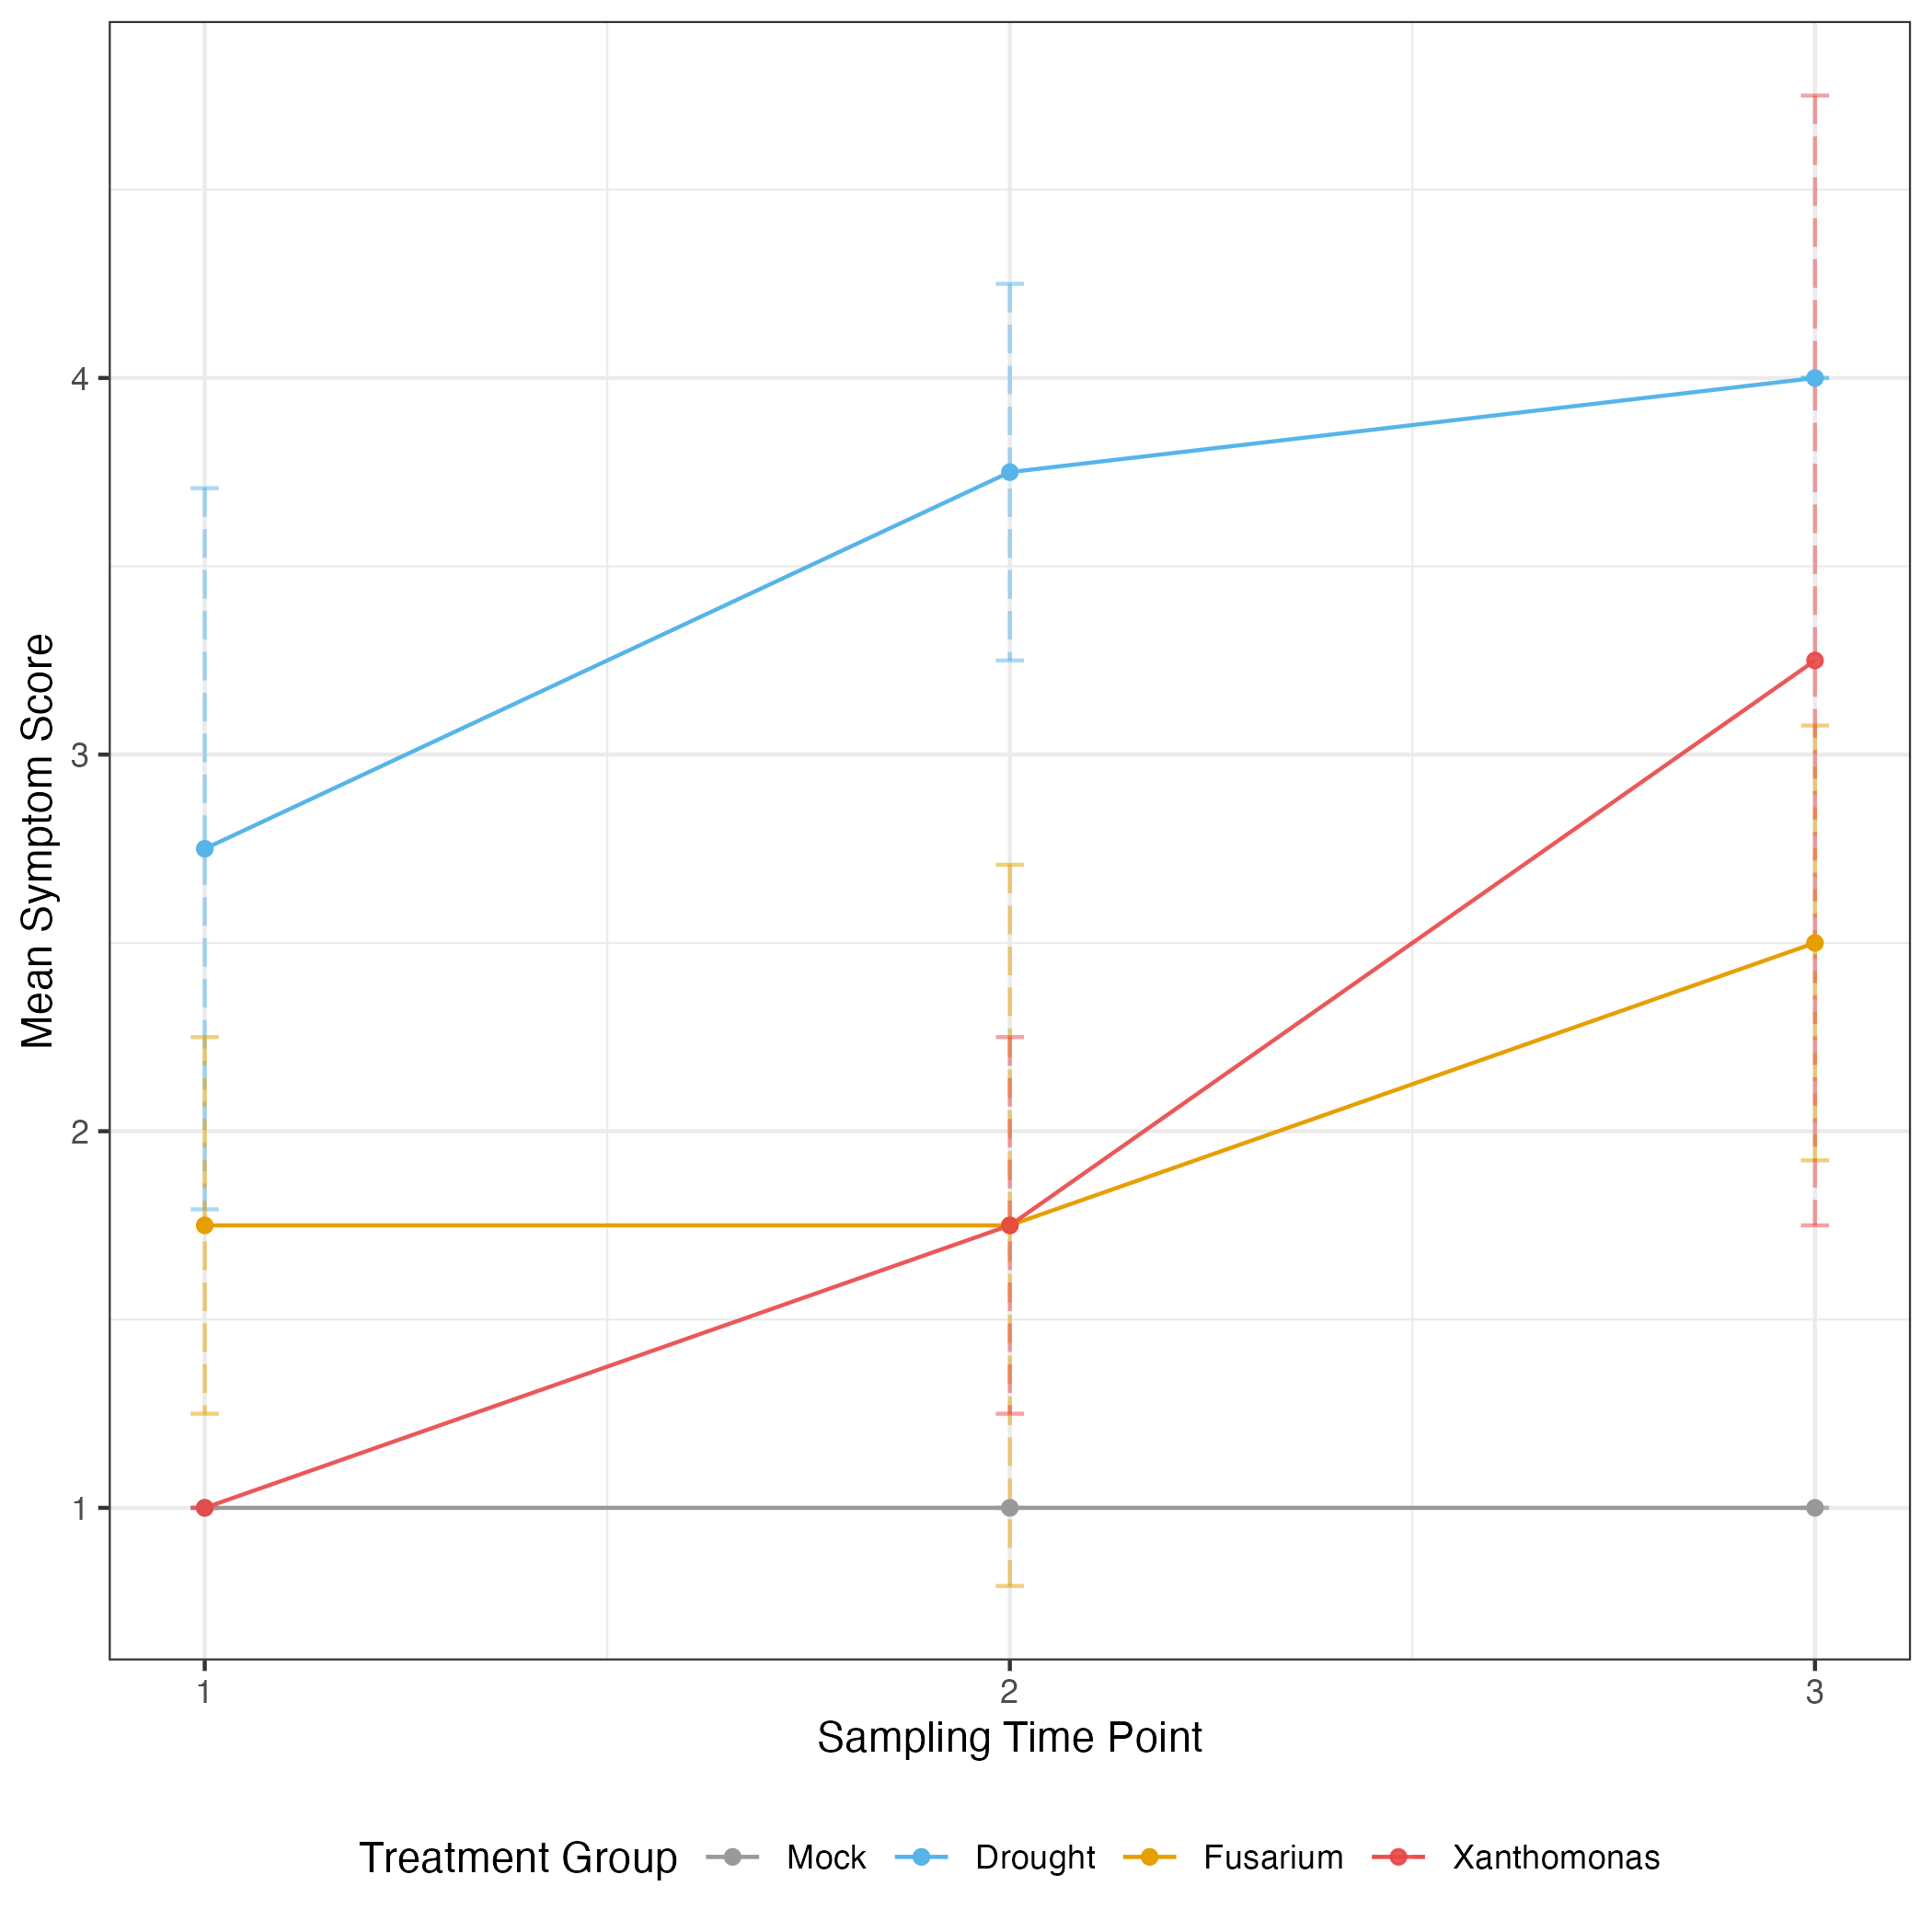
\includegraphics[width=\textwidth]{Figures/External_plot.png}
    \captionsetup{width=\textwidth}
    \caption[External symptom development scores of 'Grand Naine' plants infected with \acl{Focub4} or \acl{xvm} or subjected to drought stress]{\textbf{External symptom development scores of 'Grand Naine' plants infected with \acf{Focub4} or \acf{xvm} or subjected to drought stress show \ac{xvm} symptoms progress faster than \ac{Focub4}.} Error bars show standard deviation.}
    \label{fig:ExternalSymptoms}
\end{figure}

\begin{figure}[h!]
    \centering
    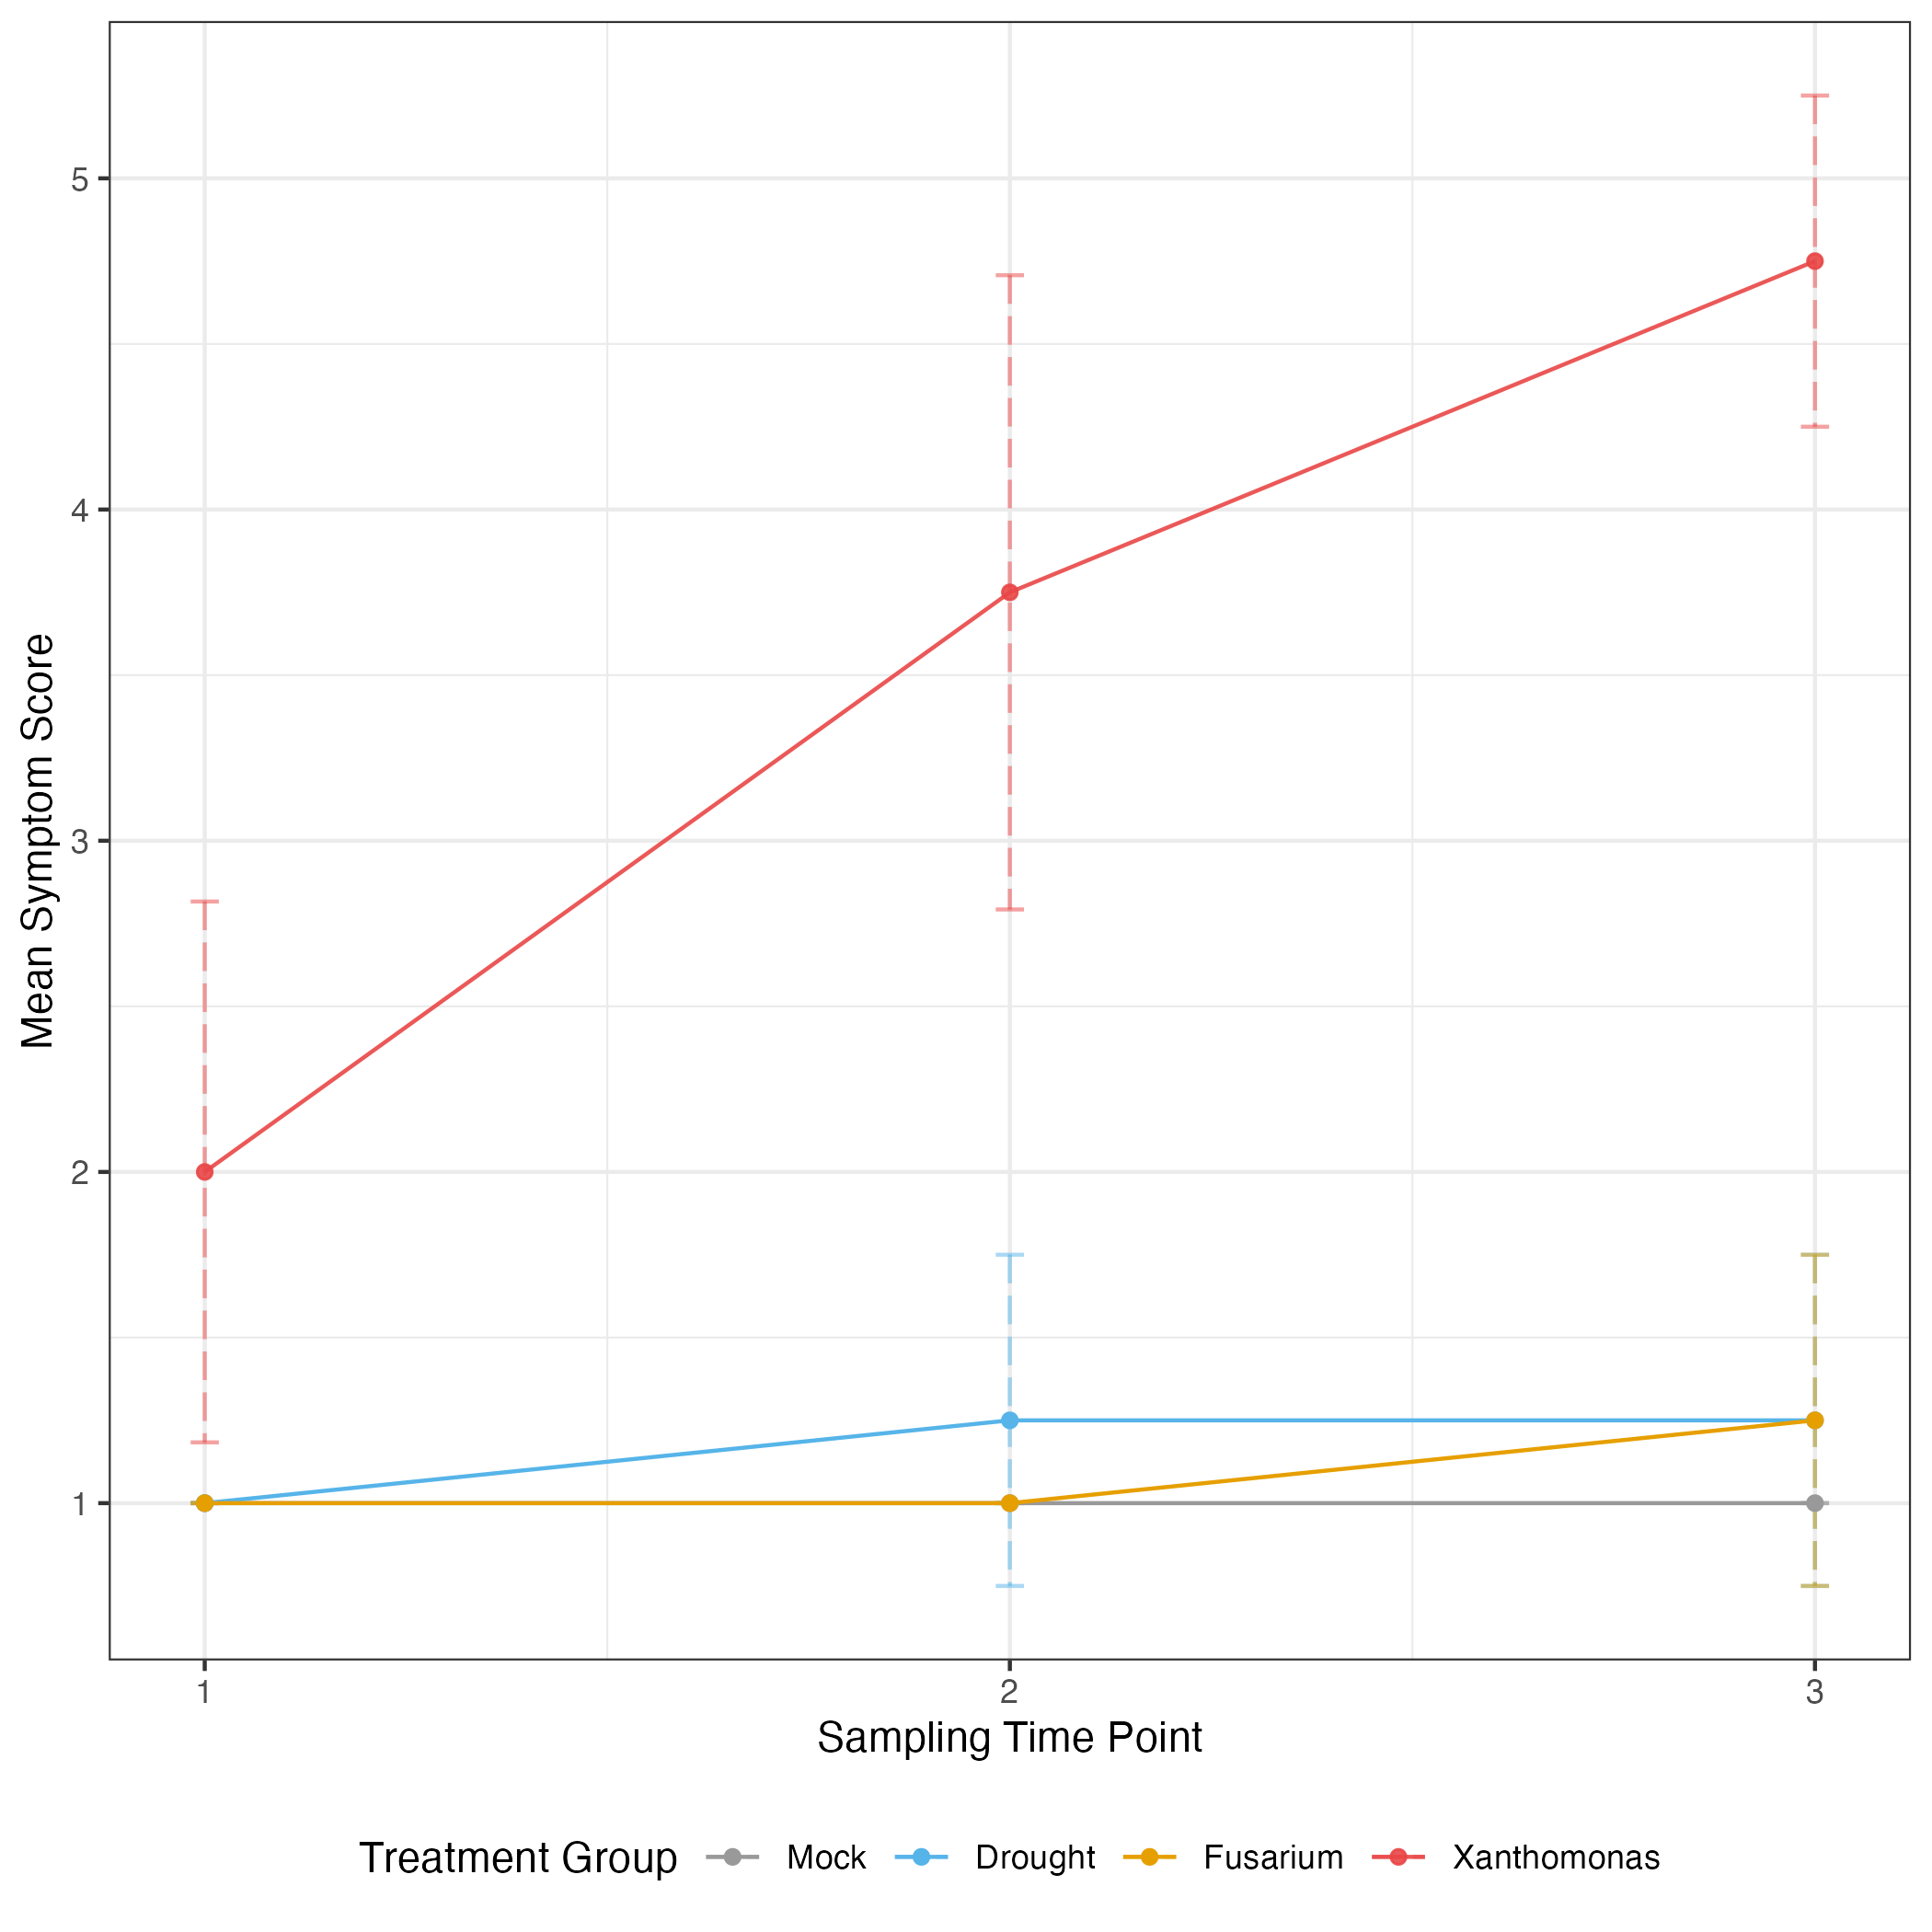
\includegraphics[width=\textwidth]{Figures/Internal_plot.png}
    \captionsetup{width=\textwidth}
    \caption[Internal symptom development scores of 'Grand Naine' plants infected with \acl{Focub4} or \acl{xvm} or subjected to drought stress]{\textbf{Internal symptom development scores of 'Grand Naine' plants infected with \acf{Focub4} or \acf{xvm} or subjected to drought stress.} Error bars show standard deviation.}
    \label{fig:InternalSymptoms}
\end{figure}

\subsection{Multispectral imaging as an approach for early symptom detection.}

Multispectral imaging represents a promising approach for the early detection of symptoms in plant pathology. Despite our rigorous analysis, we were unable to discern any significant differences between the various treatments before the naked eye.  \textcolor{red}{I need to show the images here and talk about the lack of obvious difference.} This suggests that further refinement or complementary techniques may be necessary to enhance the sensitivity of multispectral imaging for early symptom detection in our experimental setup. 

\subsubsection{Multispectral imaging does not distinguish symptoms between different wilting stresses.}

One of the primary objectives of this study was to investigate whether multispectral imaging could differentiate between different types of wilting stresses. However, our findings indicate that multispectral imaging did not effectively distinguish between the symptoms induced by various wilting stresses. \textcolor{red}{Here I can talk about the time of symptom development, but need to remember for discussion that growers are unlikely to image over time and the environmental factors will affect the speed of disease progression too quickly to make this a viable option.}
This underscores the complexity of symptom manifestation and suggests the need for alternative approaches or additional parameters to improve the discriminatory power of multispectral imaging in distinguishing between different types of wilting stresses.

\subsection{Feature distribution between treatment groups.}

To comprehensively analyse the distribution of features among treatment groups, we divided the features into distinct time points and identified features that were shared between time points, or unique to a given time point. \textcolor{red}{First, give an overview of the number of features identified in total, then the number per group. Then show the heatmap of all treatments and time points and say that basically, it's too messy to analyse the whole thing using ANOVA. Provide the ANOVA and t-test statistics for all of the time points and the treatment groups. Mention the range in the total number of significant features when comparing X against Y, and start to focus on the second time point a little more.  Then show a PCA to identify how much the treatment groups are separated by their significant feature profiles.}. 

This approach provides valuable insights into the temporal dynamics of feature expression and allows for a more nuanced understanding of the responses to different treatments over time. \textcolor{red}{Next, show the distribution of significant features across time points using a Venn diagram, and pull out some features of interest to talk about - don't go into too much detail yet because I want to see if they are shared.}


\subsection{Unique metabolites identified in the \acl{Focub4} at the second time point.}

At the second time point, the average external symptom scores recorded for \ac{Focub} and \ac{xvm} were the same (1.5). As we collected foliar samples for \ac{um} and wanted to identify features that can differentiate the two diseases, we decided to focus on significant features at the second time point and identified a set of unique features specific to the \acl{Focub4} treatment group. To elucidate the distinct metabolic signatures associated with this treatment, we\textcolor{red}{... explain how the features were grouped across treatments and show the Venn diagram with the shared and unique features between treatments at this timepoint and discuss the numbers/features of interest}. These findings highlight the potential importance of these unique metabolites in the response of \acl{Focub4}.

\subsection{Features of interest and putative identification.}

\subsubsection{Features of to distinguish abiotic and biotic stress}

\textcolor{red}{A lot of the features I have found so far separate drought from the other treatments. Can these be used to differentiate abiotic and biotic stresses? Check the heatmap and see if drought sits further back when clustering, if so - add in or refer to PCA here and look at the features of interest. What could they be? Does that have a role in stress responses?}


\subsubsection{Features of interest  from \ac{Focub} and putative identification.}
\textcolor{red}{Delve into the features of interest unique to \ac{Foucb}. Start with a dendrogram of the significant features so we can see how they fall according to the other treatment groups. See if they have similar M and T values and if they're potentially the same thing. I need to look at the fold changes and the -ve mode corroboration to see that they are genuinely due to infection too! I don't know what they are yet so harder to flesh out this section.}

\newpage
\section{Discussion and conclusion}
